\documentclass[a4paper]{scrartcl}
\usepackage[english]{babel}
\usepackage[top=2cm,bottom=3cm,left=2.5cm,right=2.5cm]{geometry}
\usepackage[colorlinks=true, allcolors=black]{hyperref}
\usepackage{wrapfig} %문단 내 이미지 삽입
\usepackage{graphicx} %색상
\usepackage{overpic}
\usepackage[normalem]{ulem}%취소선
\usepackage{array} %표
\usepackage{mdframed, tcolorbox} %글상자
\usepackage[yyyymmdd]{datetime}
	\renewcommand{\dateseparator}{--}
\usepackage{amsmath, amsfonts, amssymb, bm} %수식
	\DeclareMathOperator{\arccsc}{arccsc}
	\DeclareMathOperator{\arcsec}{arcsec}
	\DeclareMathOperator{\arccot}{arccot}
	\DeclareMathOperator{\csch}{csch}
	\DeclareMathOperator{\sech}{sech}
	\DeclareMathOperator{\arcsinh}{arcsinh}
	\DeclareMathOperator{\arccosh}{arccosh}
	\DeclareMathOperator{\arctanh}{arctanh}
	\DeclareMathOperator{\arccsch}{arccsch}
	\DeclareMathOperator{\arcsech}{arcsech}
	\DeclareMathOperator{\arccoth}{arccoth}
	
	\DeclareMathOperator{\meter}{m}
	\DeclareMathOperator{\cm}{cm}
	\DeclareMathOperator{\mm}{mm}
	\DeclareMathOperator{\mum}{\mu m}
	\DeclareMathOperator{\newton}{N}
	\DeclareMathOperator{\kn}{kN}
	\DeclareMathOperator{\kgf}{kgf}
	\DeclareMathOperator{\pa}{Pa}
	\DeclareMathOperator{\kpa}{kPa}
	\DeclareMathOperator{\mpa}{MPa}
	\DeclareMathOperator{\gpa}{GPa}
	\DeclareMathOperator{\npm}{N/m}
	\DeclareMathOperator{\knpm}{kN/m}
	\DeclareMathOperator{\kph}{km/h}
	\DeclareMathOperator{\mps}{m/s}
	\DeclareMathOperator{\tkph}{kph}
	\DeclareMathOperator{\tmps}{mps}
	\DeclareMathOperator{\mpss}{m/s^2}
	\DeclareMathOperator{\dgr}{\!^\circ}
	\DeclareMathOperator{\cel}{\!^\circ C}
	\DeclareMathOperator{\kg}{kg}
	\DeclareMathOperator{\kgpcm}{kg/m^3}
	\DeclareMathOperator{\nm}{N\cdot m}
	\DeclareMathOperator{\knm}{kN\cdot m}
	\DeclareMathOperator{\kw}{kW}
	\DeclareMathOperator{\kwh}{kWh}
	\DeclareMathOperator{\mmhg}{mmHg}
	\DeclareMathOperator{\snd}{s}
\usepackage{polynom} %나눗셈 필산
\usepackage{cancel} %수식 약분선
\usepackage{titlesec} %섹션 이름 변경
	\titlespacing*{\section}{3mm}{0mm}{1mm}
	\titleformat{\section}{\bfseries\large}{}{0ex}{}
\usepackage{kotex} %한글

\newcommand{\prob}[2]{\section{#1}\begin{mdframed}#2\end{mdframed}}

\newlength{\picwidth}
\newcommand{\probpic}[4]{
	\setlength{\picwidth}{145mm}\addtolength{\picwidth}{-#3}\section{#1}\begin{mdframed}\begin{tabular}{m{#3}m{\picwidth}}
	\includegraphics[width = #3]{#2} & #4\end{tabular}\end{mdframed}
	}

\title{\vspace{100pt}\Huge{HW4}}
\author{
	2025-2 구조역학(박성훈 교수님)\\[10pt]
	Problem 9.95, 9.102, 9.103, 9.109, 9.110\\[100pt]
	오류 제보\quad eusnoohong03@soongsil.ac.kr\\
	}
\date{\today}

\begin{document}
	
\renewcommand*{\titlepagestyle}{empty}
\maketitle

\vspace{60pt}

\begin{center}
	\includegraphics[width=0.45\textwidth]{SSU symbol KR-EN.jpg}
\end{center}

\newpage\setcounter{page}{1}

\setlength{\parindent}{0pt}

\textsf{\textbf{Use the moment-area method to solve the following problems.}}\\

\probpic{Problem 9.95}{img/p095.png}{47mm}{For the uniform cantilever beam and loading shown, determine ($a$) the slope at the free end, ($b$) the deflection at the free end.}
\begin{tabular}{m{45mm}m{115mm}}
	\includegraphics{img/fig001.png}
	&
	$\displaystyle A_m = M_0L,\quad \bar{x} = \frac{L}{2}$\newline\newline
	$\displaystyle \theta_{A/B} = \theta_{A} = -\frac{A_m}{EI} = -\frac{M_0L}{EI} \quad\blacktriangleleft\quad(a)$\newline\newline
	$\displaystyle t_{A/B} = y_A = \frac{A_m\bar{x}}{EI} = \frac{M_0L^2}{2EI}\quad\blacktriangleleft\quad(b)$
\end{tabular}
	
\vspace{20pt}

\probpic{Problem 9.102}{img/p102.png}{70mm}{For the cantilever beam and loading shown, determine ($a$) the slope at point $A$, ($b$) the deflection at point $A$. Use $E = 200\gpa$.}
$$I = 40.1\times10^6\mm^4 = 40.1\times10^{-6}\meter^4$$
Case 1,\\
\begin{tabular}{m{60mm}m{110mm}}
	\quad\includegraphics[width = 50mm]{img/fig003.png}\newline\newline
	\includegraphics{img/fig002.png}
	&
	$V_A = 0$\newline\newline
	$\displaystyle M_C = -(26\knpm)(2.7\meter)(1.35\meter) = 94.77\knm$\newline\newline
	$\displaystyle A_{m1} = \frac{1}{3}(94.77)(2.7)\knm^2 = 85.293\knm^2$\newline\newline
	$\displaystyle \bar{x}_1 = \frac{3}{4}(2.7\meter) = 2.025\meter$\newline\newline
	$\displaystyle \theta_{A/C,1} = \theta_{A1} = \frac{A_{m1}}{EI} = 10.63504\times10^{-3}$\newline\newline
	$\displaystyle t_{A/C,1} = y_{A1} = -\frac{A_{m1}\bar{x}_1}{EI} = -21.5360\mm$\\
	\quad
\end{tabular}

Case 2,\\
\begin{tabular}{m{60mm}m{110mm}}
	\quad\includegraphics[width = 50mm]{img/fig003-1.png}
	&
	$\text{In portion $AB$,}\quad V = 0$\newline\newline
	$\displaystyle M_C = (18\kn)(2.2\meter) = 39.6\knm$
\end{tabular}

\newpage

\begin{tabular}{m{60mm}m{110mm}}
	\includegraphics{img/fig004.png}
	&
	$\displaystyle A_{m2} = \frac{1}{2}(39.6)(2.2)\knm^2 = 43.56\knm^2$\newline\newline
	$\displaystyle \bar{x}_2 = \frac{2}{3}(2.2\meter) + 0.5\meter = \frac{59}{30}\meter$\newline\newline
	$\displaystyle \theta_{A/C,2} = \theta_{A2} = -\frac{A_{m2}}{EI} = -5.43142\times10^{-3}$\newline\newline
	$\displaystyle t_{A/C,2} = y_{A2} = \frac{A_{m2}\bar{x}_2}{EI} = 10.68180\mm$\\
	\quad
\end{tabular}
\begin{align*}
	&\theta_A = \theta_{A1} + \theta_{A2} = 5.20\times10^{-3}\quad\blacktriangleleft\quad(a)\\
	&y_A = y_{A1} + y_{A2} = -10.85\mm\quad\blacktriangleleft\quad(b)
\end{align*}

\vspace{20pt}

\probpic{Problem 9.103}{img/p103.png}{70mm}{Two C150$\times$12.2 channels are welded back to back and loaded as shown. Knowing that $E = 200\gpa$, determine ($a$) the slope at point $D$. ($b$) the deflection at point $D$.}
$$P = 5\kn,\quad I = 2\times5.45\times10^6\mm^4 = 10.9\times10^{-6}\meter^4$$
For a single concentrated load $P$ that is applied at $x=L$(point $E$),\\[10pt]
	\begin{tabular}{m{55mm}m{105mm}}
		\includegraphics{img/fig005.png}
		&
		$\displaystyle A_{m} = \frac{PL^2}{2},\quad \bar{x} = \frac{2L}{3}$\newline\newline
		$\displaystyle \theta_{E/A} = \theta_{E}(L) = -\frac{A_{m}}{EI} = -\frac{PL^2}{2EI}$\newline\newline
		$\displaystyle t_{E/A} = y_{E}(L) = -\frac{A_{m}\bar{x}}{EI} = -\frac{PL^3}{3EI}$
	\end{tabular}

	Use superpositions.
	\begin{align*}
		\theta_D &= \theta_{E}(0.6\meter) + \theta_{E}(1.2\meter) + \theta_{E}(1.8\meter) = -5.78\times10^{-3}\quad\blacktriangleleft\quad(a)\\
		y_D &= y_{E}(0.6\meter) + 1.2\meter\cdot\theta_{E}(0.6\meter) + y_{E}(1.2\meter) + 0.6\meter\cdot\theta_{E}(1.2\meter) + y_{E}(1.8\meter)\\
		&= -7.43\mm \quad\blacktriangleleft\quad(b)
	\end{align*}

\newpage

\probpic{Problem 9.109}{img/p109.png}{55mm}{For the prismatic beam and loading shown, determine ($a$) the slope at end $A$, ($b$) the deflection at the center $C$ of the beam.}
	In portion $AC$,\\[10pt]
	\begin{tabular}{m{55mm}m{105mm}}
		\includegraphics{img/fig006.png}
		&
		$\displaystyle A_m = \frac{PL^2}{16},\quad \bar{x} = \frac{2}{3}\left(\frac{L}{2}\right) = \frac{L}{3}$\newline\newline
		$\displaystyle \theta_{A/C} = \theta_A = -\frac{A_m}{EI} = -\frac{PL^2}{16EI} \quad\blacktriangleleft\quad(a)$\newline\newline
		$\displaystyle -t_{A/C} = y_C = -\frac{A_m\bar{x}'}{EI} = -\frac{PL^3}{48EI} \quad\blacktriangleleft\quad(b)$
	\end{tabular}

\vspace{20pt}

\probpic{Problem 9.110}{img/p110.png}{55mm}{For the prismatic beam and loading shown, determine ($a$) the slope at end $A$, ($b$) the deflection at the center $C$ of the beam.}
	In portion $AC$,\\[10pt]
	\includegraphics{img/fig007.png}
	\begin{align*}
		&A_m = \frac{1}{2}(Pa)(a) + Pa\left(\frac{L}{2}-a\right) = \frac{Pa}{2}\left(L-a\right)\\
		&\bar{x}'= \frac{L}{2} - \bar{x} = \frac{A_t\bar{x}'_t + A_s\bar{x}'_s}{A_m} = \frac{\frac{Pa^2}{2}\cdot \frac{2a}{3} + Pa\left(\frac{L}{2}-a\right)\cdot\left\{\frac{1}{2}\left(\frac{L}{2}-a\right) + a\right\}}{\frac{Pa}{2}(L-a)} = \frac{3L^2 - 4a^2}{12(L-a)}\\
		&\theta_{A/C} = \theta_A = -\frac{A_m}{EI} = -\frac{Pa(L-a)}{2EI} \quad\blacktriangleleft\quad(a)\\
		&t_{A/C} = y_C = -\frac{A_m\bar{x}'}{EI} = \frac{Pa(4a^2 - 3L^2)}{24EI} \quad\blacktriangleleft\quad(b)
	\end{align*}

\end{document}